\documentclass[a4paper,11pt]{article}

\usepackage[utf8]{inputenc}
\usepackage[british]{babel}
\usepackage{graphicx}
\usepackage{float}
\graphicspath{ {images/} }

\begin{document}
\title{FIT3036 --- Project Specification}
\author{Dylan Pinn --- 24160547}
\maketitle
\pagebreak

\tableofcontents
\pagebreak

\section{Introduction}

\section{Project Requirements}

\subsection{Functional Requirements}

\subsection{Non-functional Requirements}

\section{Project Plan}

\subsection{Overview}

\textbf{Project objectives:} Our company secured a contract for a local council in Victoria to re-surface roads in a designated square kilometre area.

Can use:
Google Maps and related
Satellite/aerial views
Work out the total area of roads in the nominated square kilometre to give a quote.
Need to write related code along with an elegant GUI to support the calculations.

Requirements:
Use any method to calculate the total area of the roads.
Has to be testable.
Easy to use GUI.

Constraints:
Only have access to publicly available data.
Available information online
No / Limited access to council records

\subsection{Risk Analysis}

% TODO: Attach Google Docs sheet and expand

\subsection{Resource Requirements}

\subsection{Schedule}

Created a Gantt Chart, as seen in figure \ref{fig:gantt}, from our Trello board using TeamGantt. This allows working back from the due date to meet deadlines.

\begin{figure}[H]
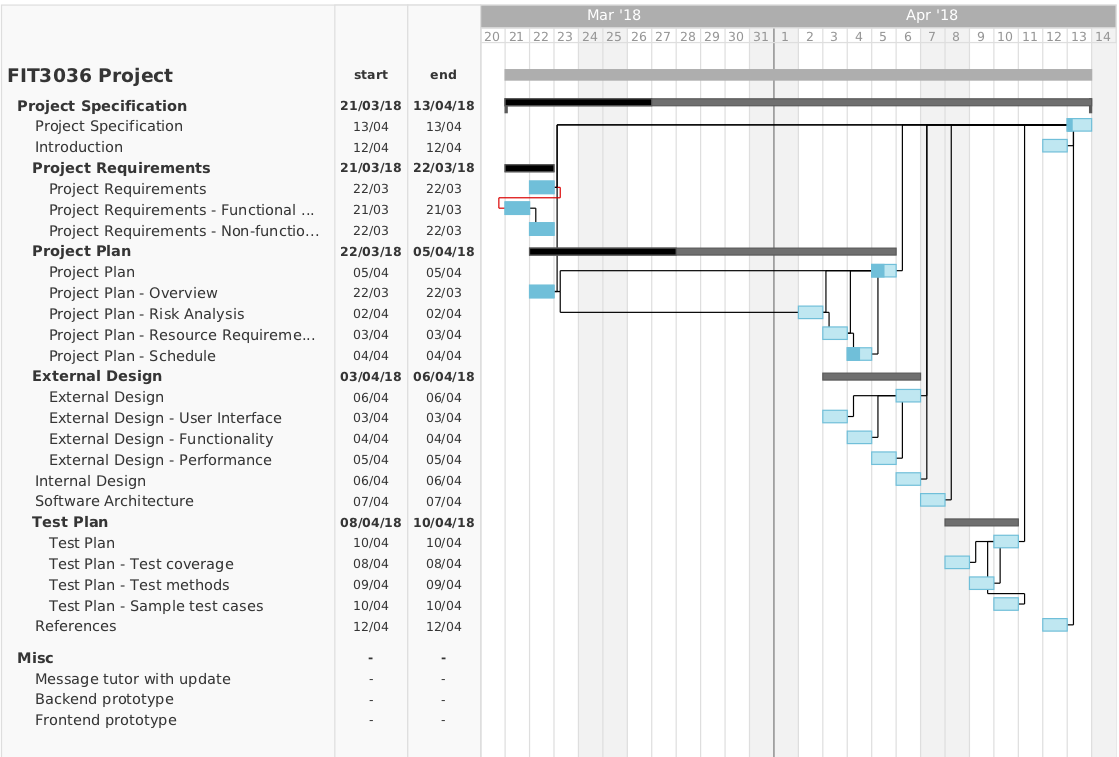
\includegraphics[width=\textwidth]{gantt-chart}
\caption{Gantt chart}
    \label{fig:gantt}
\end{figure}


\section{External Design}

\subsection{User Interface}

Created mockup figure \ref{fig:mockup}. %TODO: Add square to mockup.

Open webpage and presented with a large render of Google Maps. There is a square that can be positioned and sized over the map for the user to select the area to calculate.

A calculation shows the total area of the shape over the map.

The user then pushes the "Calculate" button to generate the surface area of the roads within the square.

There is help information on the page.

\begin{figure}[H]
  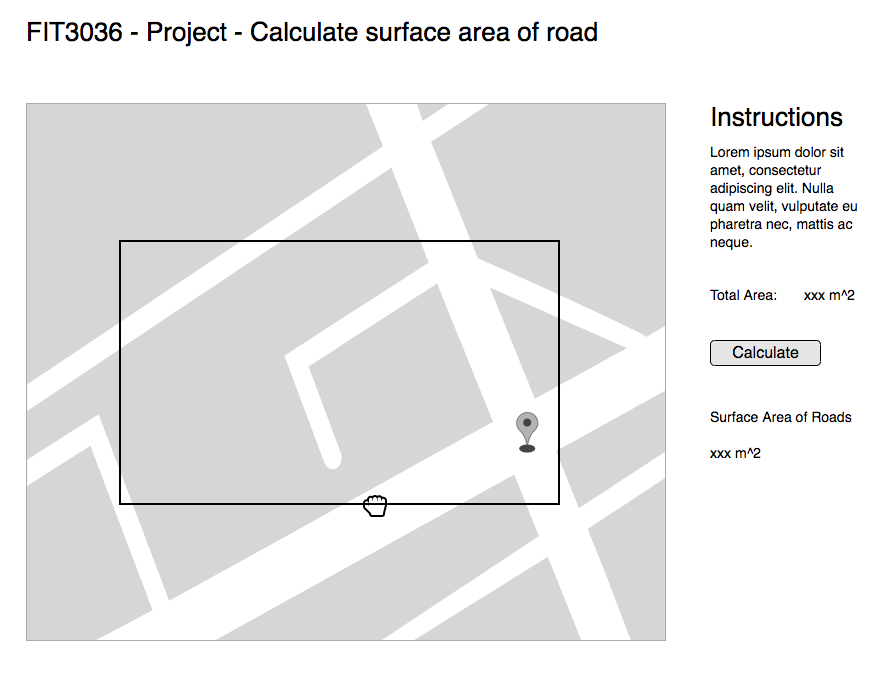
\includegraphics[width=\textwidth]{UI-mockup}
  \caption{Application Mockup}
  \label{fig:mockup}
\end{figure}

\subsection{Functionality}

\subsection{Performance}

\section{Internal Design}

\section{Software Architecture}

\section{Test Plan}

\subsection{Test coverage}

\subsection{Test methods}

\subsection{Sample test cases}

\section{References}

\end{document}
